\section{Comparison with empirical portfolio returns}
\label{sec:comparison_returns}

With the definition of the four different distributions we proceed to compare
them with empirical data from 200 stocks traded in the S\&P 500 stock market
index.

As described in Sect. \ref{sec:exact_distributions}, we obtain normalized all
the time series in the market data, the we compute the covariance matrix and
obtain the corresponding eigenvalues and eigenvectors. Using them we rotate and
scale the returns, and finally, we aggregate the rotated and scaled returns
into a single univariate distribution.

In Fig. \ref{fig:gg_dist} we plot four Gaussian-Gaussian distributions with
fit parameter $N = 2, 3, 4, 5$. The best fit seems to be the distributions
with $N = 3$ and $N = 4$.

\begin{figure}[htbp]
    \centering
    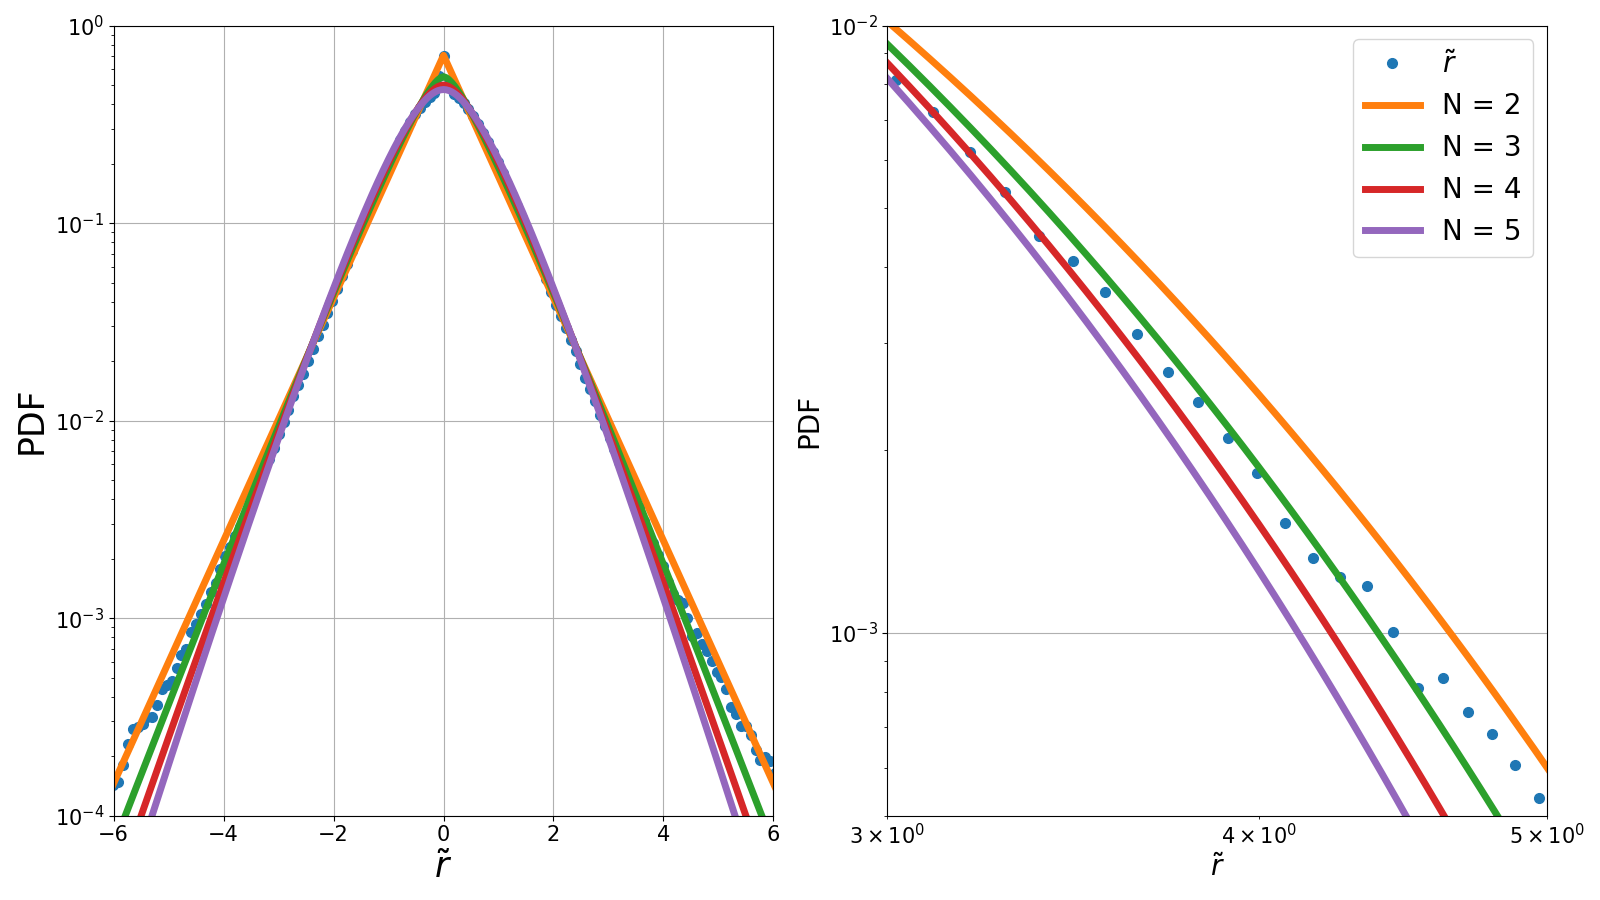
\includegraphics[width=0.7\columnwidth]
    {figures/08_gg.png}
    \caption{Gaussian-Gaussian probability density
             $\left\langle p \right\rangle_{GG'}^{\left(k\right)}$, in the
             Markovian case, normalized to unit standard deviation for
             different values of $N$, and aggregated distribution returns
             $\left(\tilde{r}\right)$ for fixed covariance for $200$ companies
             selected from the S\&P 500 dataset and $\Delta t = 1d$. (left)
             semilog scale and (right) loglog scale.}
    \label{fig:gg_dist}
\end{figure}

For the Gaussian-Algebraic distribution and Algebraic-Gaussian distribution,
we have to add an additional shape parameter $L$ and $l$, respectively. In
Fig. \ref{fig:ga_dist} we plot four Gaussian-Algebraic distributions and in
Fig. \ref{fig:ag_dist} we plot four Algebraic-Gaussian distributions with fit
parameters $N = 2, 3, 4, 5$. In both cases, a good agreement when $N = 4$ can
be seen.

\begin{figure}[htbp]
    \centering
    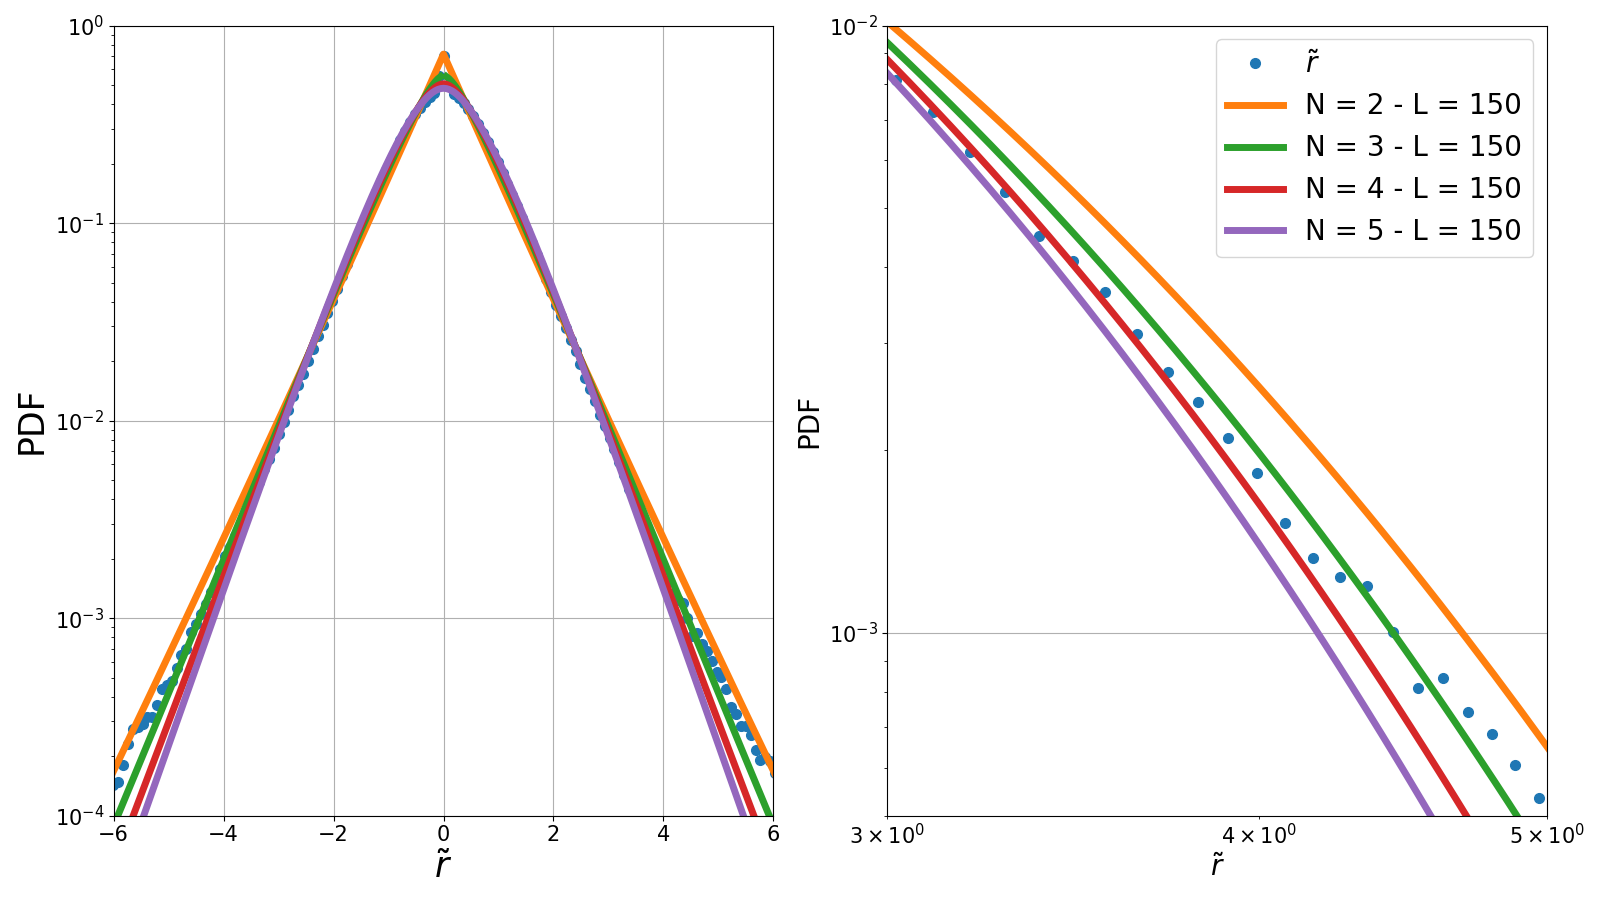
\includegraphics[width=0.7\columnwidth]
    {figures/08_ga.png}
    \caption{Gaussian-Algebraic probability density
             $\left\langle p \right\rangle_{GA'}^{\left(k\right)}$, in the
             Markovian case, normalized to unit standard deviation for
             different values of $N$, and aggregated distribution returns
             $\left(\tilde{r}\right)$ for fixed covariance for $200$ companies
             selected from the S\&P 500 dataset and $\Delta t = 1d$. (left)
             semilog scale and (right) loglog scale.}
    \label{fig:ga_dist}
\end{figure}

\begin{figure}[htbp]
    \centering
    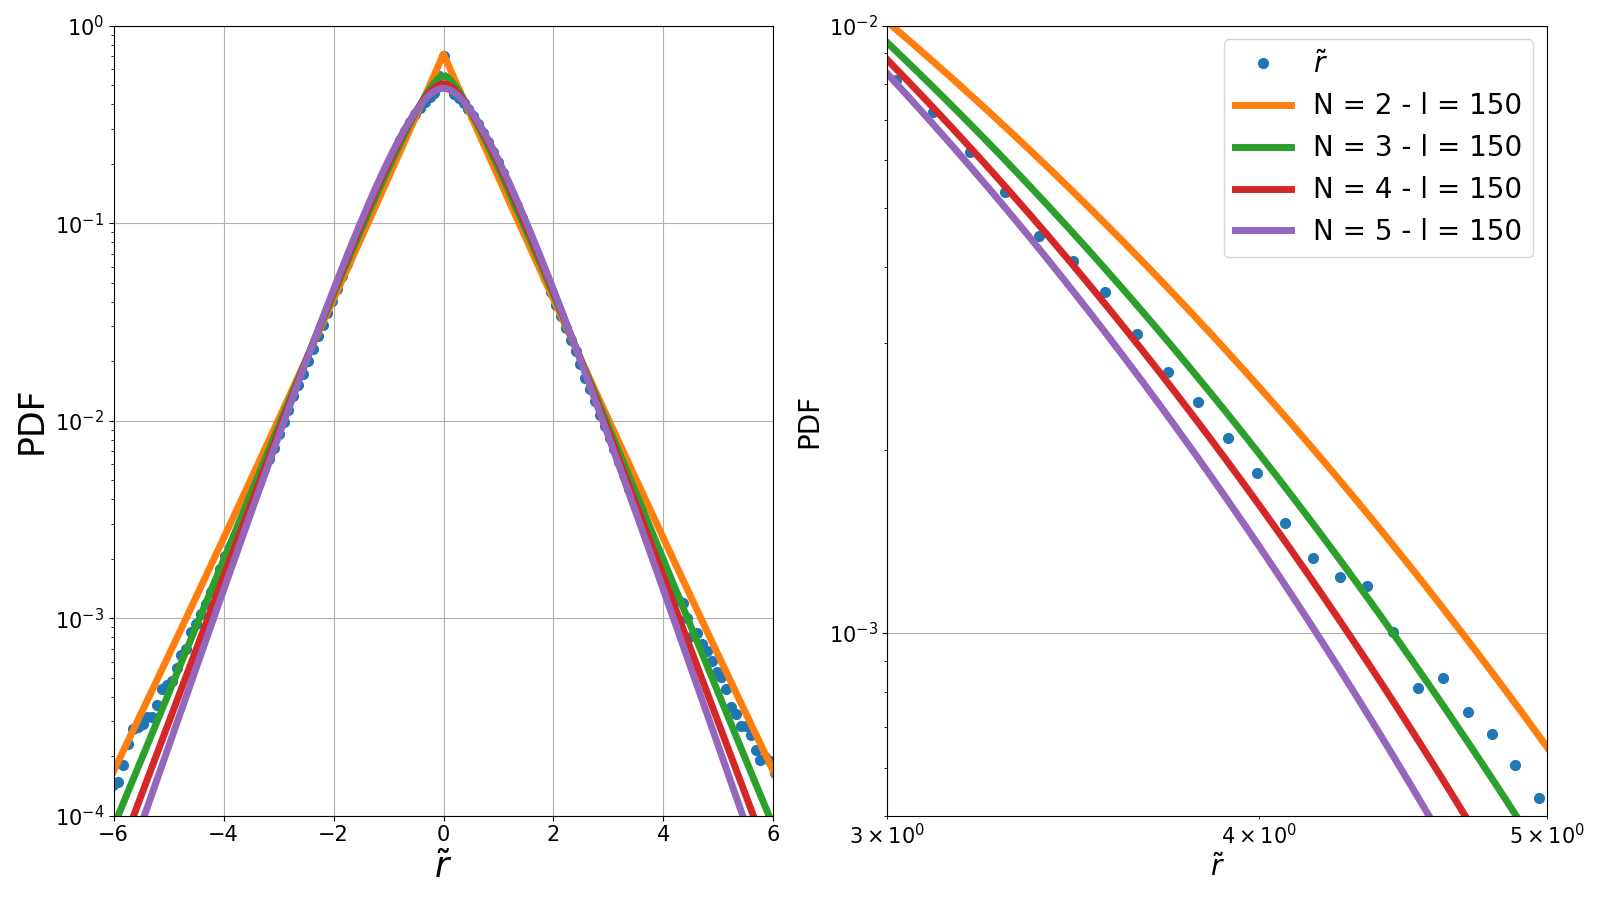
\includegraphics[width=0.7\columnwidth]
    {figures/08_ag.png}
    \caption{Algebraic-Gaussian probability density
             $\left\langle p \right\rangle_{AG'}^{\left(k\right)}$, in the
             Markovian case, normalized to unit standard deviation for
             different values of $N$, and aggregated distribution returns
             $\left(\tilde{r}\right)$ for fixed covariance for $200$ companies
             selected from the S\&P 500 dataset and $\Delta t = 1d$. (left)
             semilog scale and (right) loglog scale.}
    \label{fig:ag_dist}
\end{figure}

Finally, in Fig. \ref{fig:aa_dist} we plot four Algebraic-Algebraic
distributions with fit parameters $N = 2, 3, 4, 5$. In this case we use the
shape parameters $L$ and $l$. Again, a good agreement when $N = 4$ can be seen.

\begin{figure}[htbp]
    \centering
    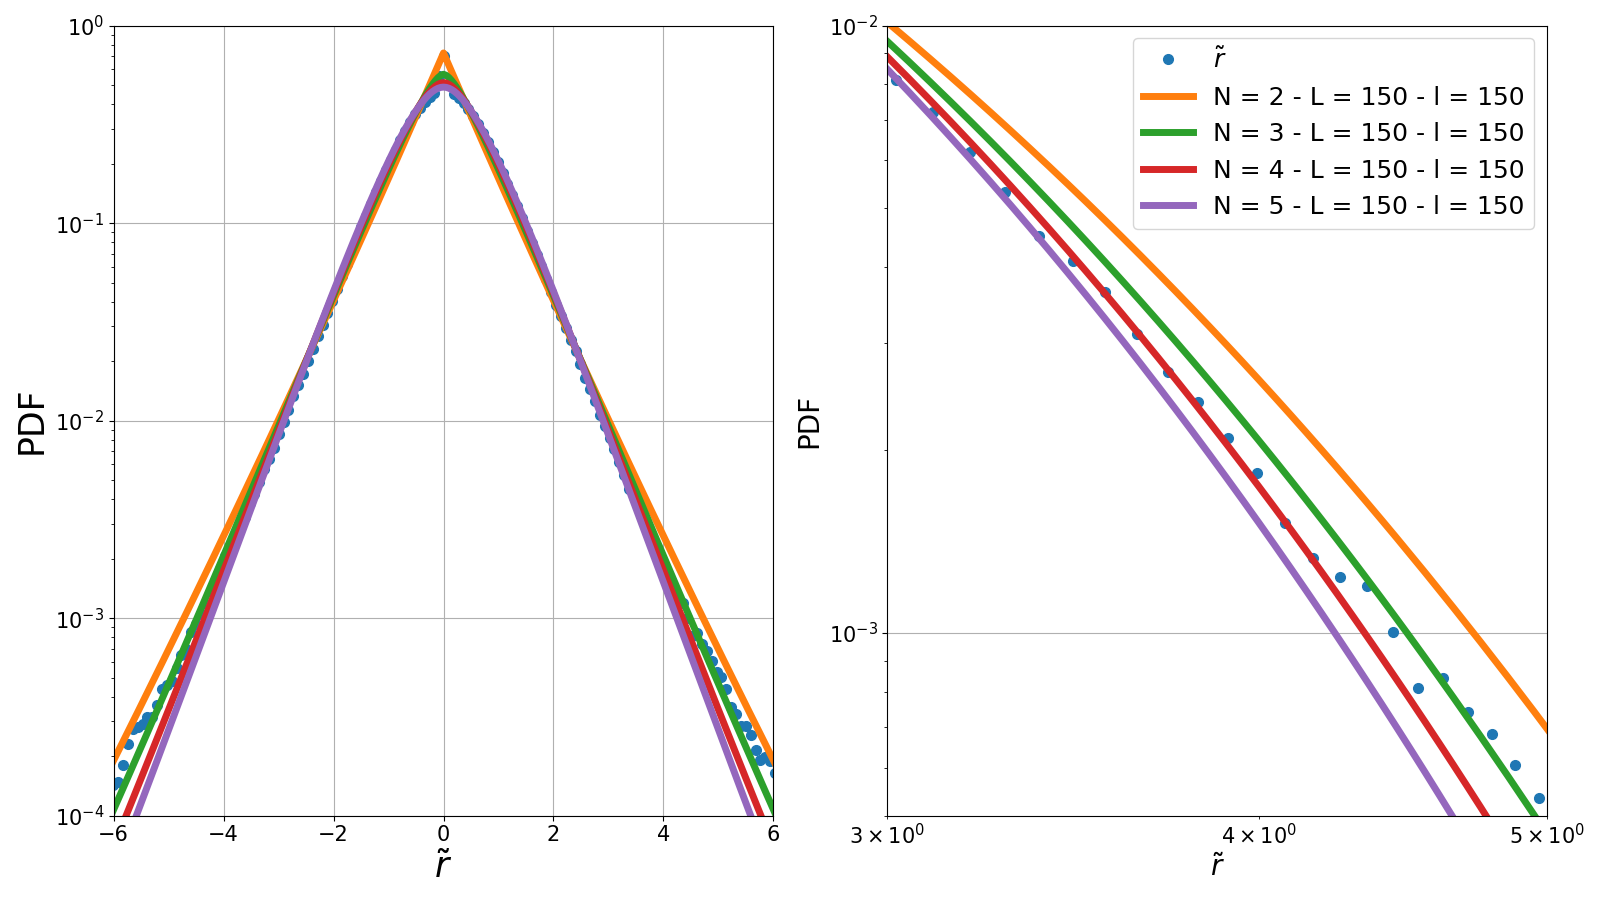
\includegraphics[width=0.7\columnwidth]
    {figures/08_aa.png}
    \caption{Algebraic-Algebraic probability density
             $\left\langle p \right\rangle_{AA'}^{\left(k\right)}$, in the
             Markovian case, normalized to unit standard deviation for
             different values of $N$, and aggregated distribution returns
             $\left(\tilde{r}\right)$ for fixed covariance for $200$ companies
             selected from the S\&P 500 dataset and $\Delta t = 1d$. (left)
             semilog scale and (right) loglog scale.}
    \label{fig:aa_dist}
\end{figure}
